\documentclass{article}
\usepackage{graphicx}
\usepackage{listings}
\usepackage{amsmath}
\usepackage{natbib}
\usepackage{fancyhdr}
%\usepackage{lastpage}

% Evita que el documento se estire verticalmente para ocupar
% el espacio vacío en cada página.
\raggedbottom

%%%%%%%%%% Configuración de Fancyhdr - Inicio %%%%%%%%%%
\pagestyle{fancy}
\thispagestyle{fancy}
\lhead{Trabajo Pr\'actico 1, Sistemas Operativos}
\rhead{Scheduling}
\renewcommand{\footrulewidth}{0.4pt}
\cfoot{\thepage /\pageref{LastPage}}

\fancypagestyle{caratula} {
   \fancyhf{}
   \cfoot{\thepage /\pageref{LastPage}}
   \renewcommand{\headrulewidth}{0pt}
   \renewcommand{\footrulewidth}{0pt}
}
%%%%%%%%%% Configuración de Fancyhdr - Fin %%%%%%%%%%

\begin{document}
%%%%%%%%%%%%%%%%%%%%%%%%%%%%%%%%%%%%%%%%%%%%%%%%%%%%%%%%%%%%%%%%%%%%%%%%%%%%%%%
%% Carátula                                                                  %%
%%%%%%%%%%%%%%%%%%%%%%%%%%%%%%%%%%%%%%%%%%%%%%%%%%%%%%%%%%%%%%%%%%%%%%%%%%%%%%%

\thispagestyle{caratula}

\begin{center}


\includegraphics[height=2cm]{images/DC.png}
\hfill

\includegraphics[height=2cm]{images/UBA.jpg}
\vspace{2cm}

Departamento de Computación,\\
Facultad de Ciencias Exactas y Naturales,\\
Universidad de Buenos Aires

\vspace{4cm}

\begin{Huge}
Trabajo Pr\'actico 1
\end{Huge}

\vspace{0.5cm}

\begin{Large}
Sistemas Operativos
\end{Large}

\vspace{1cm}

22 de Abril de 2014

\vspace{4cm}

\begin{tabular}{|c|c|c|}
    \hline
    Apellido y Nombre & LU & E-mail\\
    \hline
    Silvio Vileri\~no             & 106/12 & svilerino@gmail.com\\
    Ezequiel Gambaccini     & 715/13 & ezequiel.gambaccini@gmail.com\\
    Martin Arjovsky         & 683/12 & martinarjovsky@gmail.com\\
    \hline
\end{tabular}
\end{center}
\newpage

%%%%%%%%%%%%%%%%%%%%%%%%%%%%%%%%%%%%%%%%%%%%%%%%%%%%%%%%%%%%%%%%%%%%%%%%%%%%%%%
%% Índice                                                                    %%
%%%%%%%%%%%%%%%%%%%%%%%%%%%%%%%%%%%%%%%%%%%%%%%%%%%%%%%%%%%%%%%%%%%%%%%%%%%%%%%

\tableofcontents

\newpage

    %%%%%%%%%%%%%%%%%%%%%%%%%%%%%%%%%%%%%%%%%%%%%%%%%%%%%%%%%%%%%%%%%%%%%%%%%%%%%%%
    %% Introduccion                                                              %%
    %%%%%%%%%%%%%%%%%%%%%%%%%%%%%%%%%%%%%%%%%%%%%%%%%%%%%%%%%%%%%%%%%%%%%%%%%%%%%%%
    \section{Introducci\'on}
    El objetivo de este documento es recopilar las resoluciones de los ejercicios presentados en el enunciado del trabajo practico. En las secciones a continuaci\'on se detalla cada ejercicio.\\
    \textbf{Nota:} Los ejercicios 1, 3, 5, 6 son implementaci\'ones y no ser\'an tenidos en cuenta en la siguiente secci\'on.
    \newpage

    %%%%%%%%%%%%%%%%%%%%%%%%%%%%%%%%%%%%%%%%%%%%%%%%%%%%%%%%%%%%%%%%%%%%%%%%%%%%%%%
    %% Desarrollo                                                                %%
    %%%%%%%%%%%%%%%%%%%%%%%%%%%%%%%%%%%%%%%%%%%%%%%%%%%%%%%%%%%%%%%%%%%%%%%%%%%%%%%
    \section{Desarrollo}
        \subsection{Ejercicio 1}
Ejercicio implementado en el c\'odigo.
        \subsection{Ejercicio 2}

  A continuaci\'on se muestran los gr\'aficos del lote 2 para 1, 2 y 3 n\'ucleos.
  \begin{figure}[htb]
  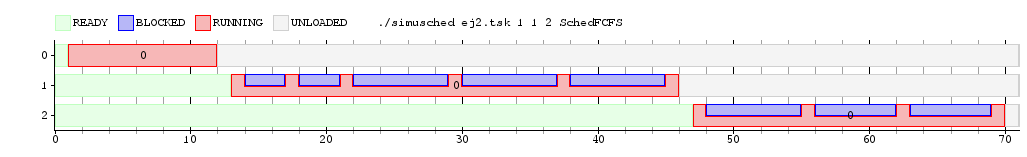
\includegraphics[scale=0.32]{images/ej2_1.png}
  \caption{Diagrama de Gantt para el lote 2 en FCFS con un n\'ucleo}
  \end{figure}
  \begin{figure}[htb]
  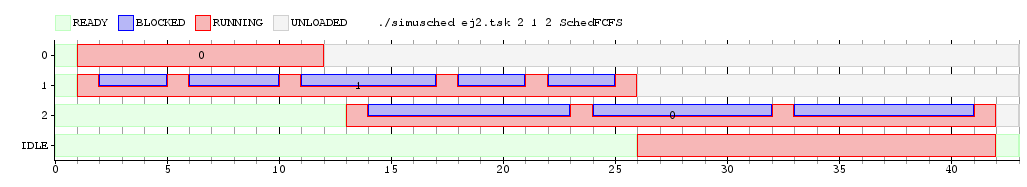
\includegraphics[scale=0.32]{images/ej2_2.png}
  \caption{Diagrama de Gantt para el lote 2 en FCFS con dos n\'ucleos}
  \end{figure}
  \begin{figure}[htb]
  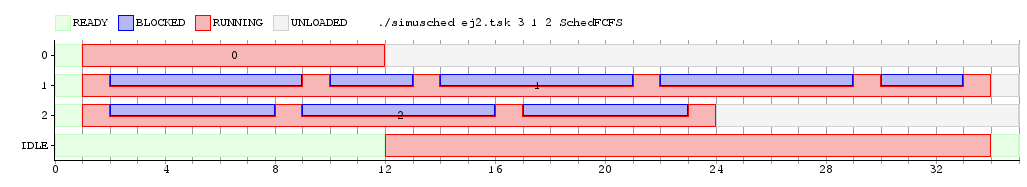
\includegraphics[scale=0.32]{images/ej2_3.png}
  \caption{Diagrama de Gantt para el lote 2 en FCFS con tres n\'ucleos}
  \end{figure}

        \subsection{Ejercicio 3}
Ejercicio implementado en el c\'odigo.
        \subsection{Ejercicio 4}

  A continuaci\'on se muestran los gr\'aficos del lote 4 ejecutado en el scheduler Round-Robin.
  \begin{figure}[htb]
  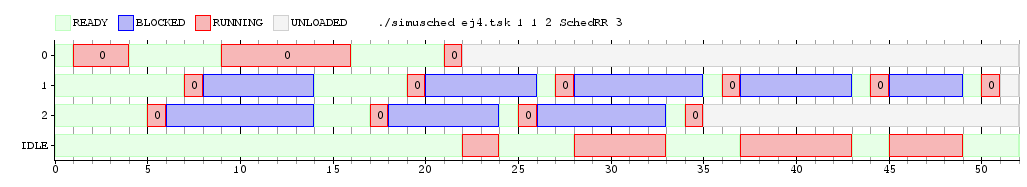
\includegraphics[scale=0.32]{images/ej4_1.png}
  \caption{Diagrama de Gantt para el lote 4 en RR con un n\'ucleo}
  \end{figure}
  \begin{figure}[htb]
  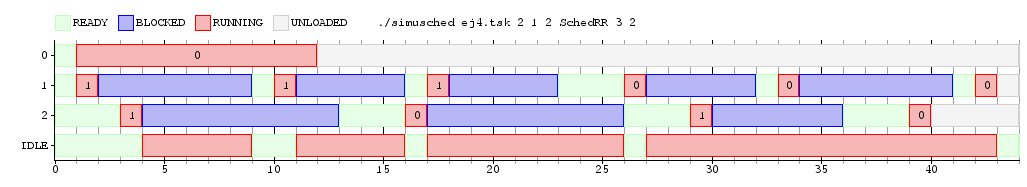
\includegraphics[scale=0.32]{images/ej4_2.png}
  \caption{Diagrama de Gantt para el lote 4 en RR con dos n\'ucleos}
  \end{figure}

  En ambos gr\'aficos se observa el comportamiento esperado de un scheduler de tipo Round-Robin. En particular, en la figura 4 se ve como la tarea 0 corre en el \'unico n\'ucleo hasta que en el tiempo 4 se le acaba
  el quantum disponible y el scheduler busca otro proceso disponible en la cola global. Tambi\'en se muestra repetidamente como cuando un proceso realiza una llamada bloqueante, el CPU deja esa tarea para ir a ejecutar
  otra. En la figura 5 se observa el mismo comportamiento, pero adem\'as podemos observar la migraci\'on de procesos entre n\'ucleos, por ejemplo a tiempo 16 en la tarea 2.

        \subsection{Ejercicio 5}
Ejercicio implementado en el c\'odigo.
        \subsection{Ejercicio 6}
Ejercicio implementado en el c\'odigo.
          \subsection{Ejercicio 7}

  Para estudiar la performance del Round-Robin variando los cuantos creamos el lote7 y realizamos varias simulaciones. Variamos los quantums entre 1 y 10 inclusive y evaluamos el throughput y INSERTAR SEGUNDA M\'ETRICA con 2 y 4 n\'ucleos. Como las tareas TaskConsola son pseudoaleatorias,
  para cada seleccio\'on de par\'ametros corrimos 10 simulaciones y graficamos el promedio con la variaci\'on estandard.

  \begin{figure}
  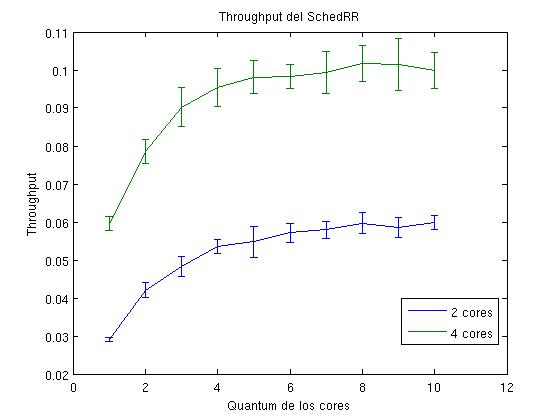
\includegraphics[scale=0.6]{images/TH.jpg}
  \caption{Throughput para SchedRR con dos y cuatro n\'ucleos}
  \end{figure}

  En la figura 6 se muestran los resultados del throughput. En la misma se observa que (considerando las desviaciones) el throughput aumenta al aumentar el quantum, tanto para 2 como 4 n\'ucleos. Esto tiene mucho sentido, ya que se
  gasta menos tiempo en cambios de contexto y es menos probable que un proceso cambie de CPU, bajando el costo total de migraci\'on de procesos entre CPUs. Obviamente, este crecimiento converge, ya que el tiempo que tardan en terminar los procesos est\'a acotado por
  el uso total del CPU dividido la cantidad de n\'ucleos, por lo que el throughput tambi\'en converge.

          \subsection{Ejercicio 8}

  A continuaci\'on se muestran los gr\'aficos del lote 8 ejecutado sobre los schedulers Round-Robin con y sin migraci\'on entre procesos.

  \begin{figure}
  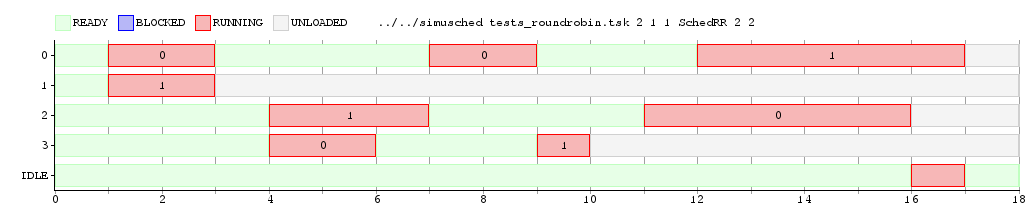
\includegraphics[scale=0.32]{images/ej8_RR.png}
  \caption{Diagrama de Gantt para el lote 8 en RR con dos n\'ucleos}
  \end{figure}

  \begin{figure}
  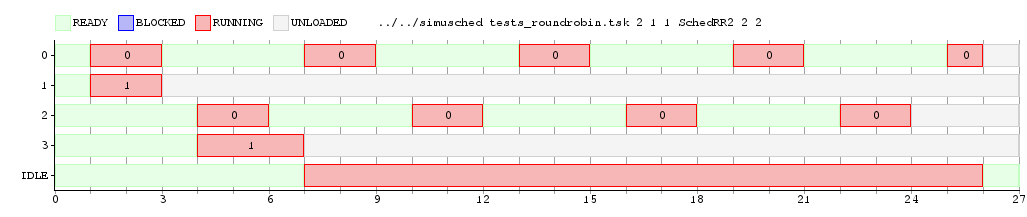
\includegraphics[scale=0.32]{images/ej8_RR2.png}
  \caption{Diagrama de Gantt para el lote 8 en RR2 con dos n\'ucleos}
  \end{figure}

  Se puede observar en el caso donde hay tareas con considerable diferencia de duracion, una mejor performance del scheduler RR1, dado que realiza una correccion permanente del balanceo de carga usando los recursos que tiene a su alcance en cada tick. Mientras que en el RR2, al quedar fija la afinidad al momento del dispatch, si ocurre un caso donde ambas tareas cortas quedan en un core y las tareas largas en otro core, al finalizar las tareas cortas, se desperdiciara un core durante toda la ejecucion de las tareas largas.
  Esta diferencia se ve claramente en los gr\'aficos 7 y 8 si notamos que cuando se usa RR1 se termina de ejecutar a tiempo 18 y con RR2 a tiempo 27, lo que es una diferencia abismal. Cabe destacar que para que esto pase se necesita
  que haya una gran diferencia entre el uso de CPU de las tareas y que las largas se encuentren concentradas en un n\'ucleo mientras las cortas en otro, lo que no suele ser un caso promedio.

        \subsection{Ejercicio 9}
Como se puede ver en los graficos de lote2 (lote2.txt, lote2rr.txt, lote2rr2.txt, lote2fcfs.txt), el unico scheduler que puede hacer que todas las tareas con deadline se realicen dentro de su limite es el EDF.
El scheduler EDF posee una propiedad que es condicion suficiente para asegurar esto, ademas de asegurar optimalidad.
Esta propiedad consiste en que si la sumatoria de la cantidad de ciclos de cada tarea divido su deadline es menor a 1, entonces el EDF va a encontrar una forma de ejecutar todas las tareas, y que además es óptima. Como se ve en los casos de las 2 implementaciones de round robin, y con el fcfs, todos fallan en lograr que todas las tareas se cumplan dentro de su deadline.
El FCFS falla al ir asignando las tareas como vienen, sin tener en cuenta nada más, por lo que al no priorizar las tareas con deadline próximos aunque hayan llegado ultimos, estos fallan.
El round robin no logra cumplir con los deadline debido a que su objetivo es tratar de balancear el uso de cpu por parte de tareas que tienen uso intesivo de cpu y tareas bloqueantes, de manera tal que no haya starvation de cpu para las tareas bloqueantes, y mientras estas estan bloqueadas, maximizar el uso de cpu, usando un quantum para mantener un balance entre las tareas. Este quantum evita que una tarea prioritaria con deadline proximo y un requirimiento de tiempo de cpu mayor a quantum se complete en el tiempo requerido.
        \subsection{Ejercicio 10}
La propiedad del edf en estos casos (lote\_edf.tsk, lote\_edf3.tsk) no se mantiene, porque aunque la suma de las tareas y sus deadlines es menor a 2, el scheduler es incapaz de hacer que se cumpla la tarea 3, aun cuando la propiedad del edf debiera ser valida.
Para mantener la propiedad de que se cumplan los deadline en un scheduler multicore, se debería usar otro algoritmo que tenga en cuenta como maximizar el uso de los procesadores, ya que para el caso de lote\_edf3.tsk, si el primer core hubiera corrido las 2 tareas de 5 y el segundo hubiese corrido la de 8, todas las tareas se habrían podido lograr en el tiempo necesario.
        \subsection{Ap\'endice: Lotes de prueba}

\lstinputlisting[caption="Lote de tests ejercicio 2", frame=single]{../codigo/experimentos/ej2.tsk}
\lstinputlisting[caption="Lote de tests ejercicio 4", frame=single]{../codigo/experimentos/ej4.tsk}
\lstinputlisting[caption="Lote de tests ejercicio 7", frame=single]{../codigo/ej7.tsk}
\lstinputlisting[caption="Lote de tests ejercicio 8", frame=single]{../codigo/experimentos/ej8/tests_roundrobin.tsk}

    %%%%%%%%%%%%%%%%%%%%%%%%%%%%%%%%%%%%%%%%%%%%%%%%%%%%%%%%%%%%%%%%%%%%%%%%%%%%%%%
    %% Conclusion                                                                %%
    %%%%%%%%%%%%%%%%%%%%%%%%%%%%%%%%%%%%%%%%%%%%%%%%%%%%%%%%%%%%%%%%%%%%%%%%%%%%%%%
    %\section{Conclusi\'on}

\end{document}